\section{Máximo Exponente de Lyapunov}
\label{sec:MLE}

El Máximo Exponente de Lyapunov (MLE) caracteriza que tan rápido se apartan dos trayectorias.
Si esta velocidad es exponencial, se dice que el sistema es caótico, por lo que este exponente es conocido como un detector de  ``caoticidad", \cite{strotgartz1994,Kantz1994,Sprott2003}.
Más adelante, el MLE fue utilizado en diversas aplicaciones de muy distintas áreas.
Sólo por mencionar alguna, en \cite{Ma2013} el MLE es usado para medir una señal muy débil en un gas ideal utilizando criterios caóticos.
En \cite{Bruijna2011}, se estudia si es posible predecir un cambio en la probabilidad de caída para un modelo simple de caminante humano a partir del $MLE$.

Los exponentes de Lyapunov son quantificadores que caracterizan como evoluciona la separación entre dos trayectorias \cite{Sprott2003}.
En general es bien conocido que el comportamiento caótico está principalmente caracterizado por los números de Lyapunov de la dinamica del sistema.
Si uno o mas números de Lyapunov es mayor que cero, entonces el sistema se comporta caóticamente, de otra forma el sistema es estable.

La distancia entre dos trayectorias cambia en $2^{MLE}$ por cada iteración, en promedio.
Si el $MLE<0$ las trayectorias se aproximan, esto puede deberse a un punto fijo.
Si el $MLE=0$ las trayectorias mantienen su distancia, esto puede deberse a un ciclo límite.
Si el $MLE>0$ la distancia entre las trayectorias es creciente, lo que es un indicador de caos.

Existe una forma no analítica de medir el $MLE$ si solo las entradas y las salidas de un sistema son accesibles.
El procedimiento es el siguiente: el sistema debe ser iniciado desde dos puntos cercanos en el plano de fase, llamémoslos $(x_a,y_a)$ y $(x_b,y_b)$.
A medida que el sistema es iterado se mide la distancia euclideana entre las dos trayectorias ($d_n$ en la muestra $n_{th}$) (eq. \ref{eq:D0D1}), y la trayectoria $b$ es relocalizada en cada iteración (eq. \ref{eq:reubicacion}) obteniendo los puntos $(x_{br},y_{br})$ para realimentar el sistema.
Entonces, el MLE puede ser calculado como se muestra en la ecuación \ref{eq:Lyapunov}.
El proceso puede verse en la Fig. \ref{fig:relocalizacion}.

\begin{eqnarray}\label{eq:D0D1}
d_{0(i-1)}&=& \sqrt{(x_{a(i-1)}-x_{br(i-1)})^2+(y_{a(i-1)}-y_{br(i-1)})^2}\nonumber\\
d_{1(i)}&=& \sqrt{(x_{a(i)}-x_{b(i)})^2+(y_{a(i)}-y_{b(i)})^2}\\
\nonumber
\end{eqnarray}

\begin{eqnarray}\label{eq:Lyapunov}
MLE &=& \frac{1}{n} \sum_{i=2}^{n} \log_2{\frac{d_{1(i)}}{d_{0(i-1)}}}
\end{eqnarray}

\begin{eqnarray}\label{eq:reubicacion}
x_{br(i)}&=& x_{a(i)}+(x_{b(i)}-x_{a(i)})d_{o(i-1)}/d_{1(i)} \nonumber\\
y_{br(i)}&=& y_{a(i)}+(y_{b(i)}-y_{a(i)})d_{o(i-1)}/d_{1(i)}
\end{eqnarray}

\begin{figure}
	\centering
	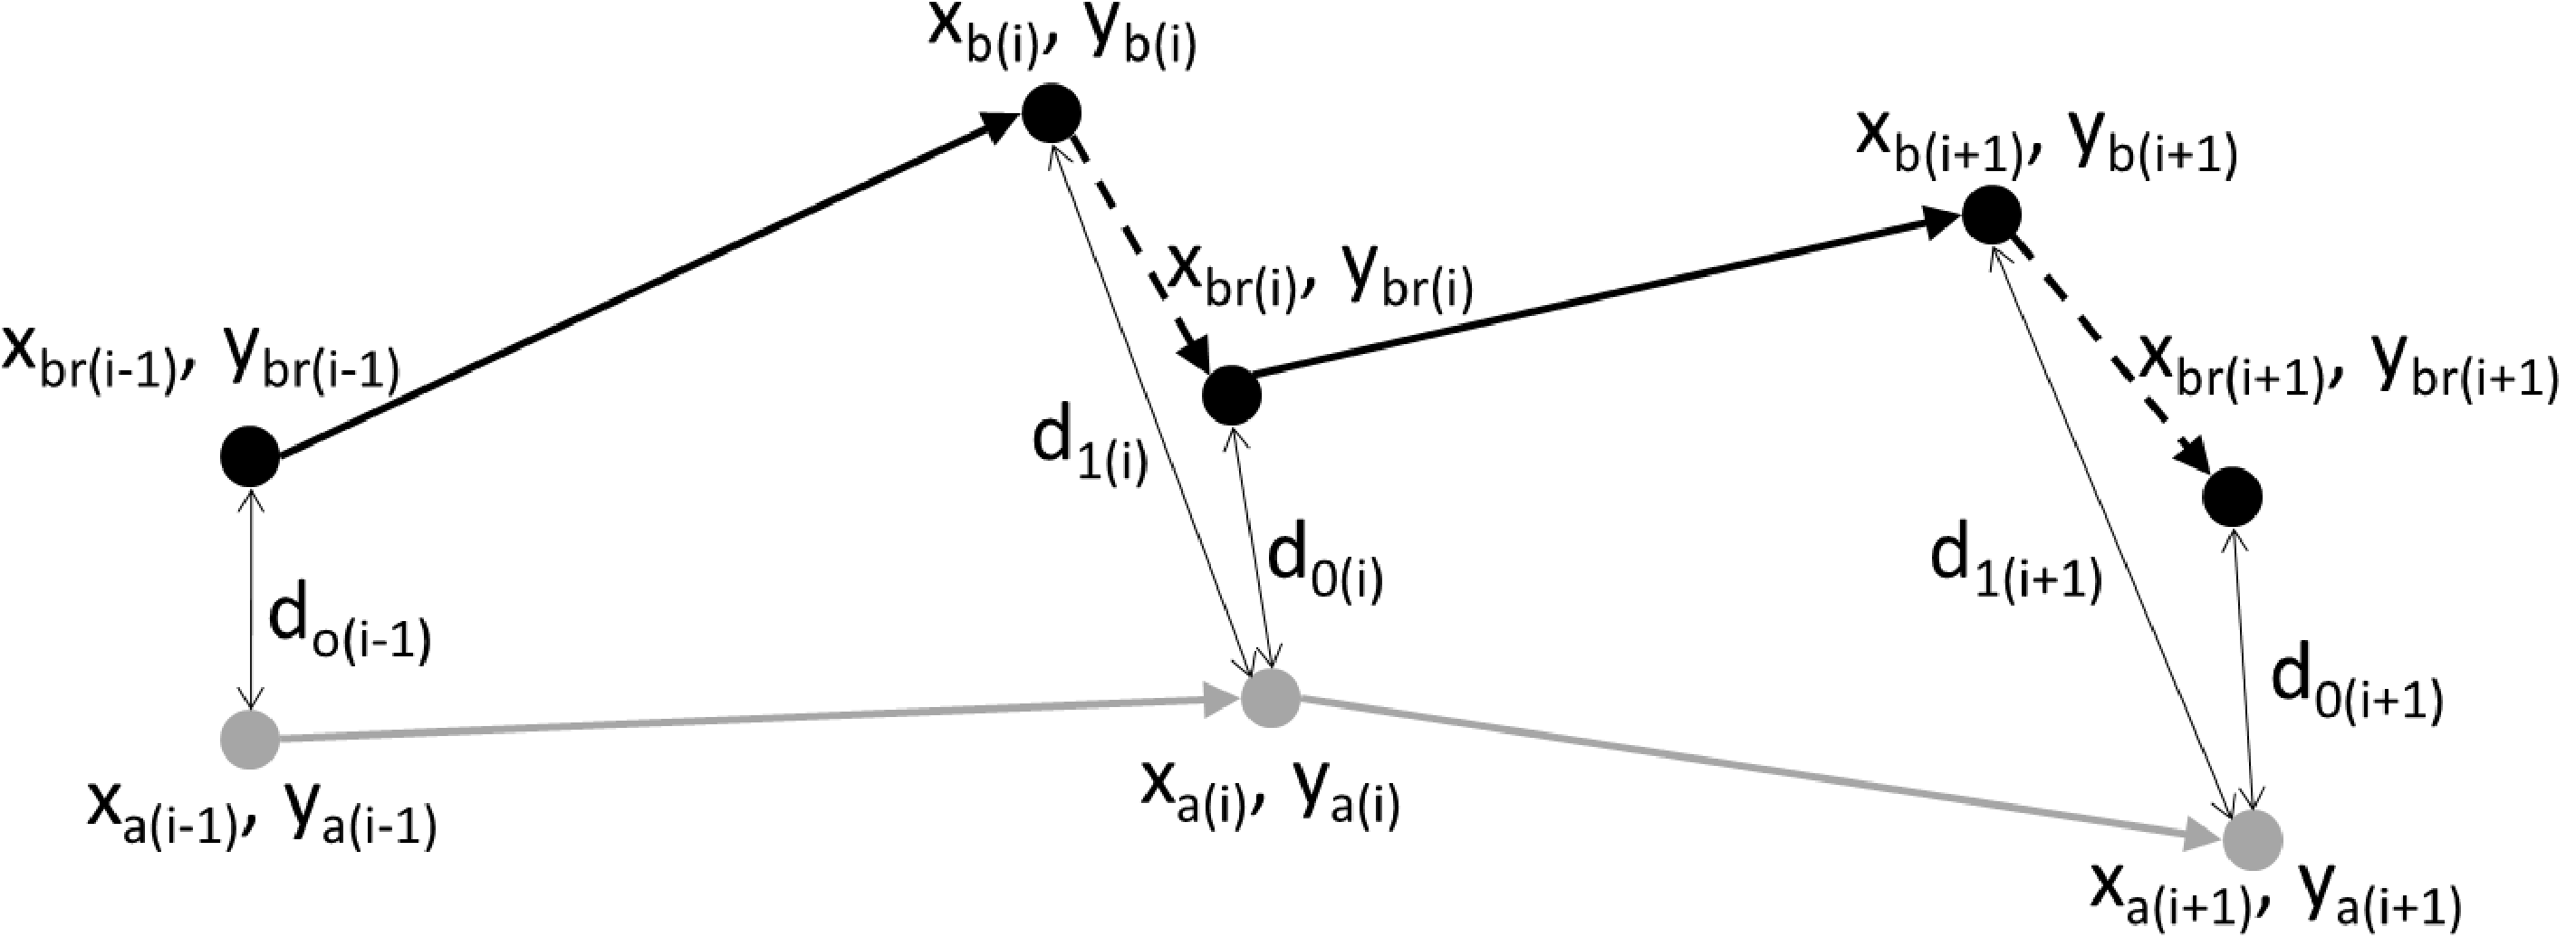
\includegraphics[width=1\columnwidth]{relocalizacion.pdf}\\
	\caption{Algoritmo para calcular el MLE.}\label{fig:relocalizacion}
\end{figure}

